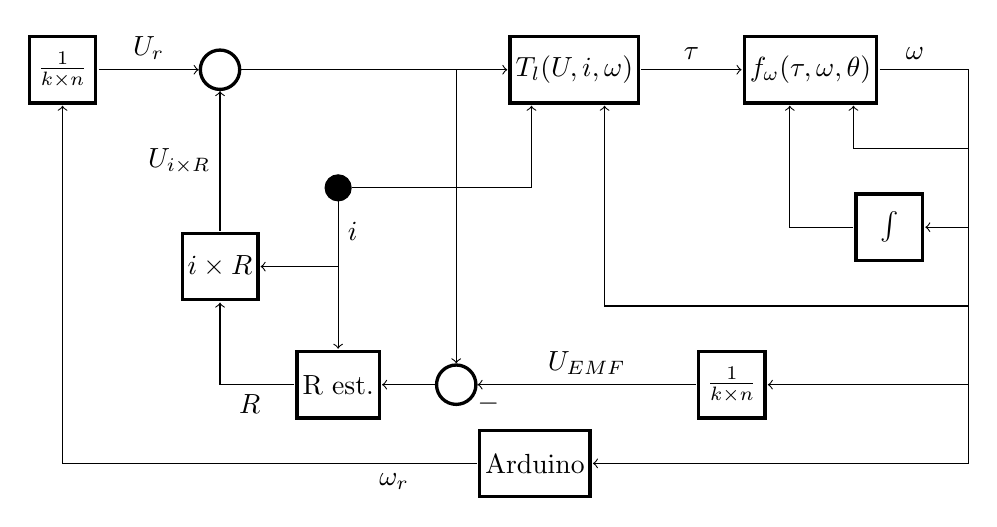
\begin{tikzpicture}
\tikzstyle{Circle} = [draw,font={\huge\bfseries}, shape=circle, minimum size=0.5cm, text=black, very thick, text width=0.2cm, align=center]
\tikzstyle{Dot} = [draw, fill, shape=circle, minimum size=0.2cm]
\tikzstyle{Block} = [draw,outer sep=1,inner sep=2,minimum size=24,line width=1, very thick]
\tikzstyle{inv} = [outer sep=0,inner sep=0,minimum size=0]
\node [Block] (v1) at (-7,3.5) {$\frac{1}{k\times n}$};
\node [Circle] (v2) at (-5,3.5) {};
\node [inv] (v8) at (4.5,0.5) {};
\node [inv] (v9) at (4.5,1.5) {};
\node [inv] (v4) at (-2,3.5) {};
\node [Block] (v5) at (-0.5,3.5) {$T_l(U,i,\omega)$};
\node [Block] (v6) at (2.5,3.5) {$f_{\omega}(\tau,\omega,\theta)$};
\node [inv] (v3) at (4.5,2.5) {};
\node [Block] (v7) at (-1,-1.5) {Arduino};
\node [Block] (v10) at (3.5,1.5) {$\int$};
\node [Block] (v12) at (1.5,-0.5) {$\frac{1}{k\times n}$};
\node [inv] (v11) at (4.5,-0.5) {};
\node [Circle] (v13) at (-2,-0.5) {};
\node [Block] (v15) at (-3.5,-0.5) {R est.};
\node [Dot] (v14) at (-3.5,2) {};
\node [Block] (v16) at (-5,1) {$i\times R$};
\draw [->] (v1) edge node[midway,above] {$U_r$} (v2);
\draw [->] (v2) edge (v5);
\draw [->] (v5) edge node[midway,above] {$\tau$} (v6);
\draw (v6) -| (v3) node[pos=0.2,above] {$\omega$};
\draw [->] (v9) -- (v8) -| (v5.-50);
\draw [->] (v8) -- (v11) -- (v12);
\draw [->] (v12) edge node[pos=0.95,below] {$-$} node[midway,above] {$U_{EMF}$} (v13);
\draw [->] (v4) edge (v13);
\draw [->](v3) -- (v9) -- (v10);
\draw [->] (v3) -| (v6.-40);
\draw [->] (v10) -| (v6.-120);
\draw [->] (v14) edge node[pos=0.2,right] {$i$} (v15);
\draw [->] (v14) |- (v16);
\draw [->] (v15) -| (v16) node[pos=0.3,below] {$R$};
\draw [->] (v16) edge node[midway,left] {$U_{i\times R}$} (v2);
\draw [->] (v13) edge (v15);
\draw [->] (v11) |- (v7);
\draw [->] (v7) -| (v1)  node[below,pos=0.1] {$\omega_r$};
\draw [->] (v14) -| (v5.-140);
\end{tikzpicture}
    